% vim:set spell tw=79:

\documentclass[beamer]{uibk}
\title{Exploitation Techniques and Mitigations}
\subtitle{Dark Arts of Computer Science}
\author{Alex Hirsch \and Patrick Ober}
\date{2016-01-15}

\usepackage{multicol}
\newminted{nasm}{fontsize=\scriptsize,frame=leftline,framesep=2mm,linenos}

\AtBeginSection[] {
    \begin{frame}{Outline}
        \begin{multicols}{2}
            \tableofcontents[currentsection]
        \end{multicols}
    \end{frame}
}

\begin{document}

\maketitle

\begin{frame}{Outline}
    \begin{multicols}{2}
        \tableofcontents
    \end{multicols}
\end{frame}

\begin{frame}{Acknowledgement}
    \begin{columns}
        \begin{column}{0.5\textwidth}
            We use a lot from RPISEC, a university course about modern
            exploitation at Rensselaer Polytechnic Institute (2015), because
            \dots

            \begin{description}
                \item<1->[of them:] They did a great job.
                \item<2->[of you:] You will see familiar material.
                \item<3->[of us:] We are lazy.
            \end{description}

            Check them out at \url{http://rpis.ec/} and
            \url{https://github.com/RPISEC/MBE}.
        \end{column}
        \begin{column}{0.5\textwidth}
            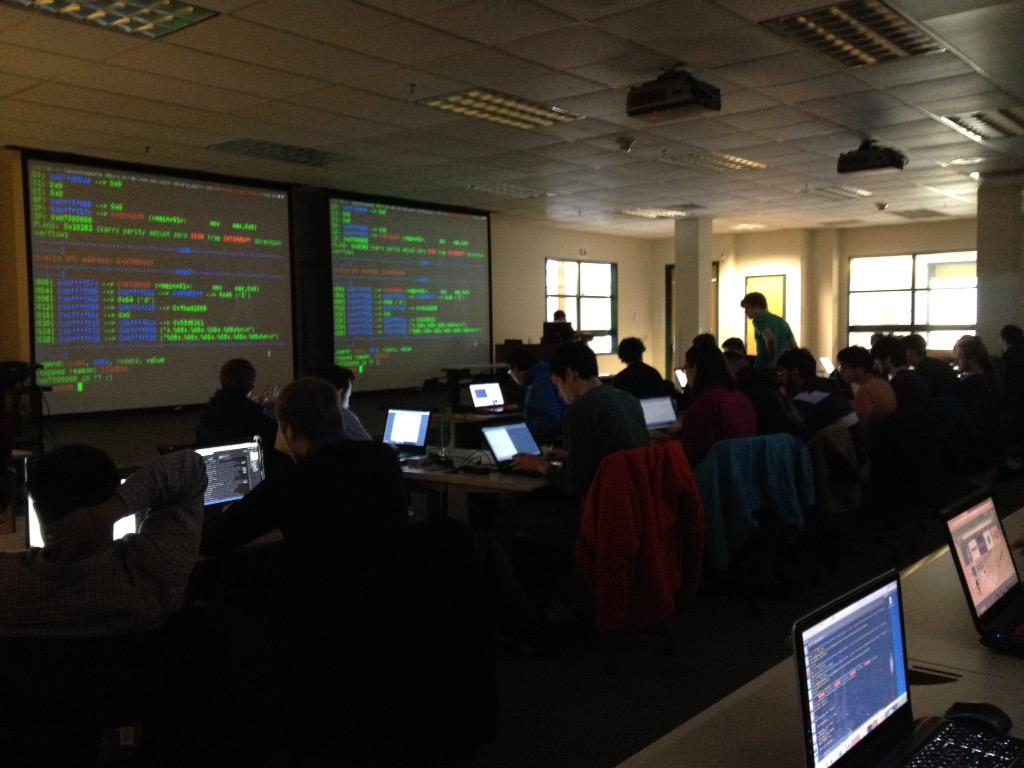
\includegraphics[height=0.7\textheight]{ripsec}
        \end{column}
    \end{columns}
\end{frame}

\section{Platform x86}

\begin{frame}{Why?}
    \begin{itemize}
        \item It's simpler, yet not overly simplified.
        \item People call it \emph{more academic} \quad *sigh*
        \item Most techniques can be translated easily.
        \item Most material covers x86.
    \end{itemize}
    \bigskip
    We are using Ubuntu 15.10 x86 inside VirtualBox here.
\end{frame}

\begin{frame}{Registers}
    \begin{center}
        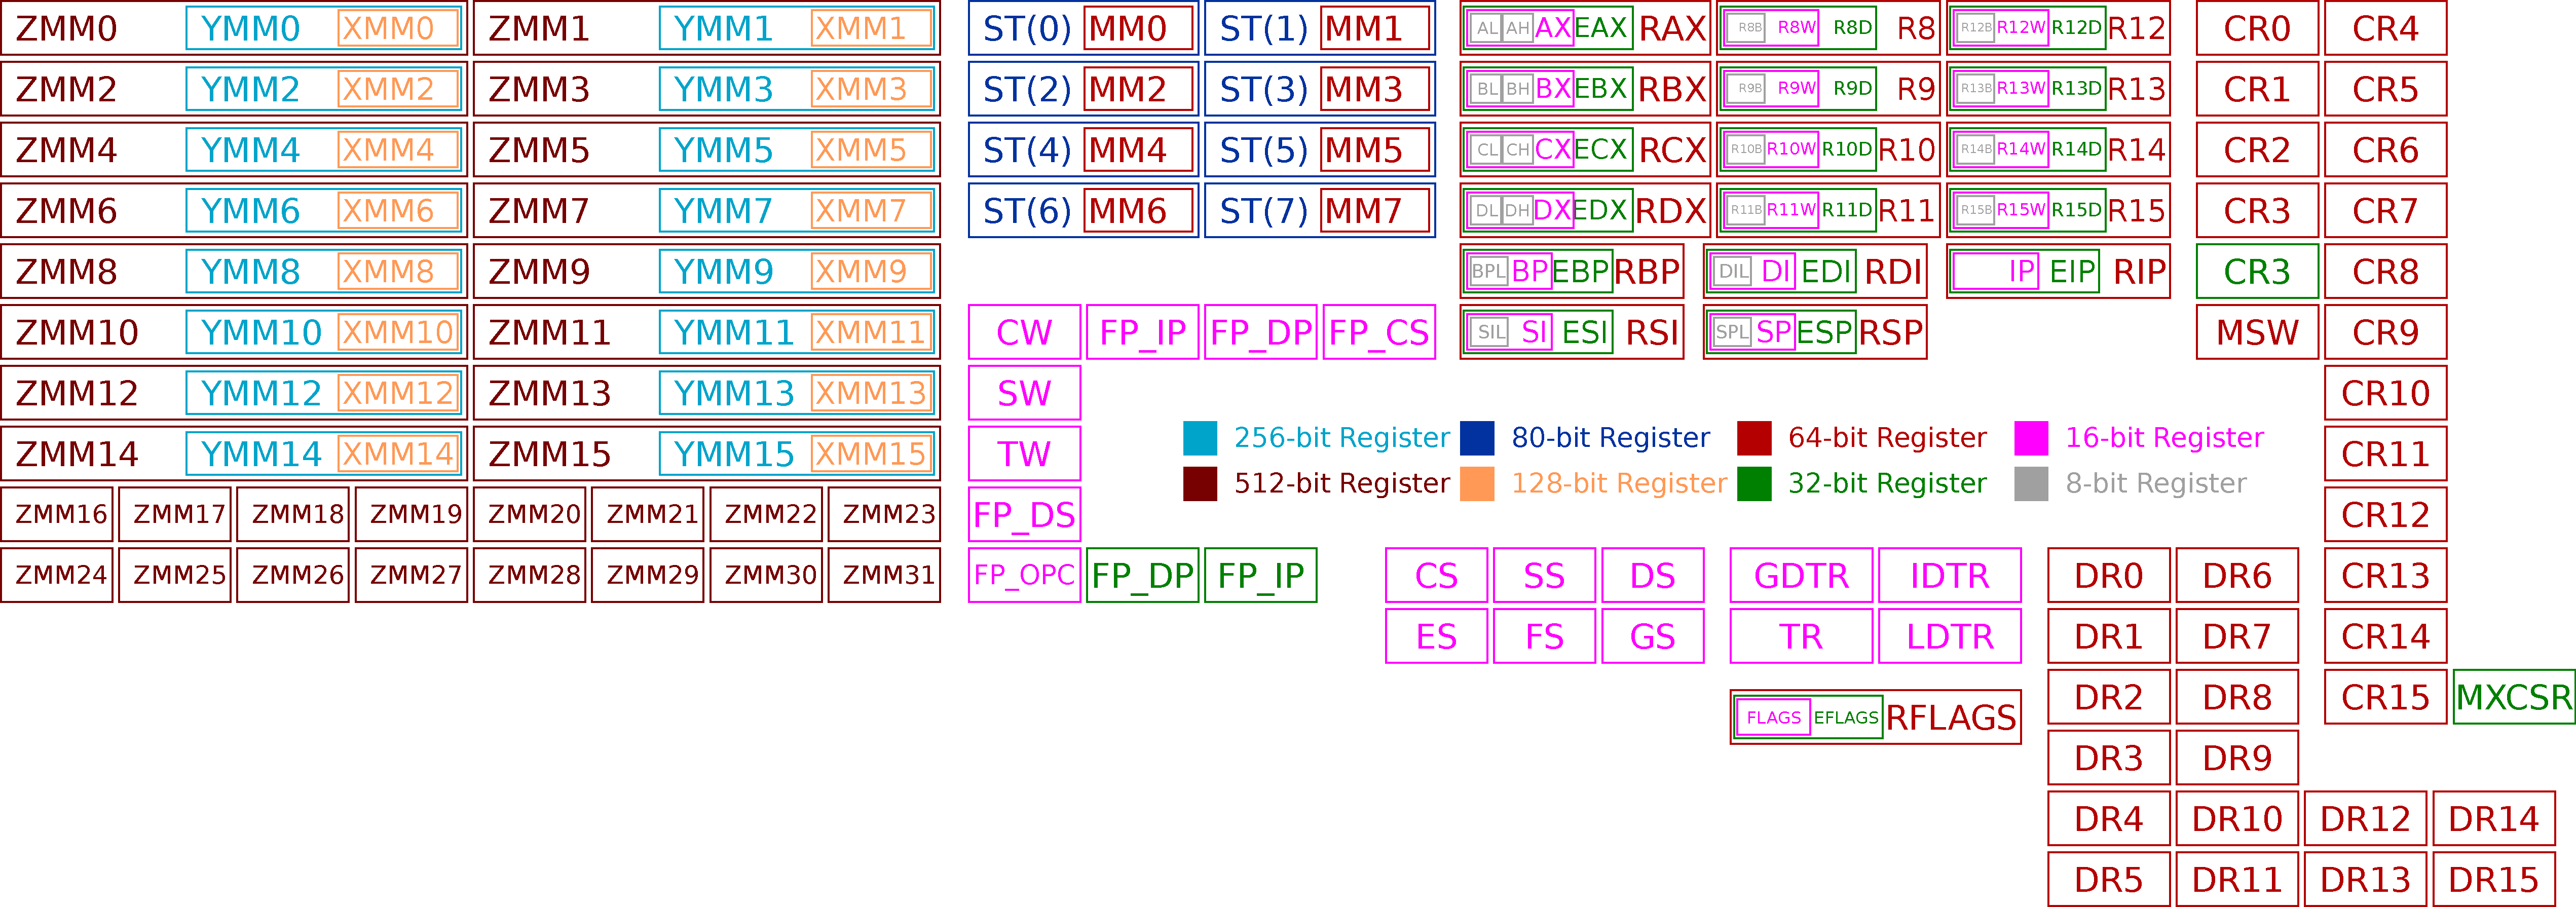
\includegraphics[width=\textwidth]{x86_registers}
    \end{center}
    \sidenote{- Wikipedia}
\end{frame}

\begin{frame}{Registers}
    \begin{center}
        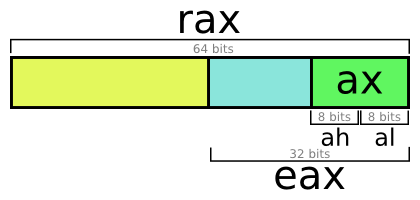
\includegraphics[height=0.5\textheight]{single_register}
    \end{center}
    \sidenote{- \url{http://nullprogram.com/}}
\end{frame}

\begin{frame}{Memory Management}
    \begin{columns}
        \begin{column}{0.45\textwidth}
            Real memory is managed by your OS kernel, a process sees only
            \textbf{virtual} memory.

            \medskip

            Memory is segmented (\textbf{pages}), which are handled by hardware
            (\textbf{memory management unit}) and software (kernel).

            \medskip

            \SI{4}{\kibi\byte} typical page size, addresses can be decomposed,
            page pointer + offset:

            $\mathtt{0xA1B2C3D4} \to \texttt{0xA1B2C000} + \mathtt{0x3D4}$
        \end{column}
        \begin{column}{0.55\textwidth}
            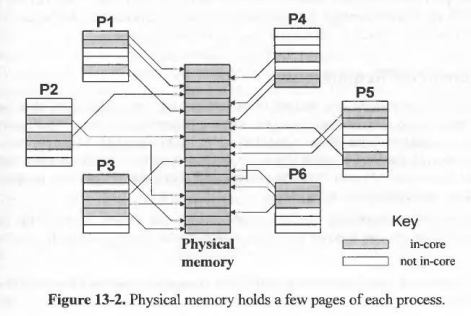
\includegraphics[height=0.7\textheight]{pages}
        \end{column}
    \end{columns}
    \sidenote{- Unix Internals by Uresh Vahalia}
\end{frame}

\begin{frame}{Process' Memory}
    \begin{columns}
        \begin{column}{0.5\textwidth}
            \begin{center}
                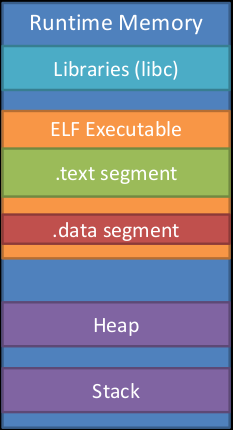
\includegraphics[height=0.8\textheight]{mem_layout}
            \end{center}
        \end{column}
        \begin{column}{0.5\textwidth}
            You know some of this, other talks also focus on this.

            \bigskip

            We'll see:
            \begin{itemize}
                \item Pages have permissions \texttt{rwx} (DEP)
                \item Layout not always the same (ASLR)
                \item Lots of pointers
            \end{itemize}
        \end{column}
    \end{columns}
\end{frame}

\begin{frame}{Calling Convention}
    \begin{columns}
        \begin{column}{0.5\textwidth}
            Defines:

            \begin{itemize}
                \item where to place arguments
                \item where to place return value
                \item where to place return address
                \item who prepares the stack
                \item who cleans afterwards\\
                    (caller vs.\ callee)
            \end{itemize}

            \pause

            Depends on:

            \begin{itemize}
                \item your platform
                \item your toolchain (language)
                \item your settings (compiler flags)
            \end{itemize}

        \end{column}

        \pause

        \begin{column}{0.5\textwidth}
            I know, Radu never told you\dots

            \medskip

            \textbf{C Declaration (cdecl):}

            \begin{itemize}
                \item arguments on stack (reverse order)\\
                    aligned to \SI{16}{\byte} boundary
                \item return via register (\texttt{EAX} / \texttt{ST0})
                \item return address on stack\\
                    (old instruction pointer \texttt{IP})
                \item old base pointer \texttt{BP}
                \item caller does the cleanup
            \end{itemize}
        \end{column}
    \end{columns}
\end{frame}

\begin{frame}[fragile]{System Call \& Protection Rings}
    \begin{columns}
        \begin{column}{0.55\textwidth}
            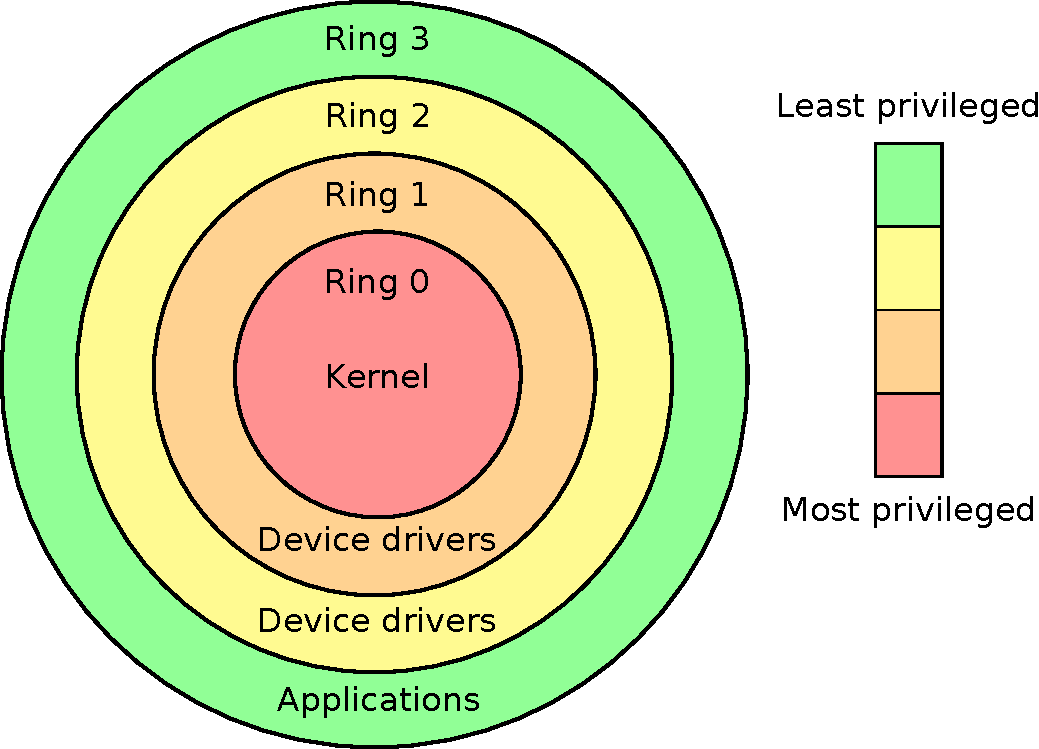
\includegraphics[width=\textwidth]{x86_rings}
        \end{column}
        \begin{column}{0.45\textwidth}
            Your CPU can switch from a more privileged state to a less
            privileged one.

            \bigskip

            Kernel does not run always, process cannot do everything (enforced
            by hardware).

            \bigskip

            Process uses a \emph{System Call} (own instruction) to notify the
            kernel to take over (context switch).

            \begin{nasmcode*}{autogobble,linenos=false}
                int   0x80   ; old, but still works
                call  write  ; new: sysenter via VDSO
            \end{nasmcode*}
        \end{column}
    \end{columns}
    \sidenote{- Wikipedia}
\end{frame}

\begin{frame}{System Calls}
    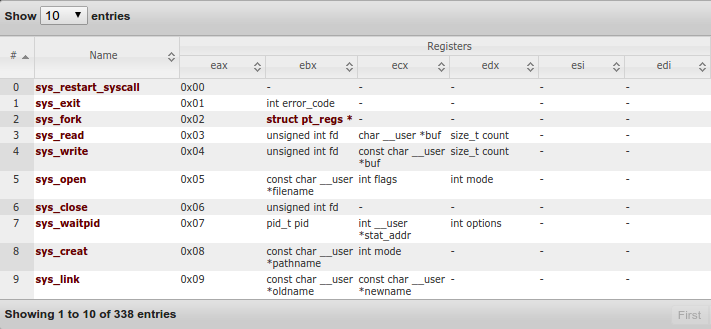
\includegraphics[width=\textwidth]{systemcalls}
    \sidenote{- \url{http://syscalls.kernelgrok.com/}}
\end{frame}

\begin{frame}{Endianness}
    \begin{columns}
        \begin{column}{0.5\textwidth}
            \begin{center}
                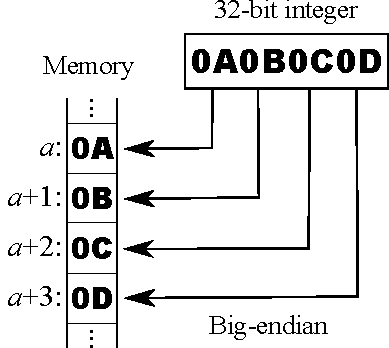
\includegraphics[width=0.8\textwidth]{big_endian}
            \end{center}
        \end{column}
        \begin{column}{0.5\textwidth}
            \begin{center}
                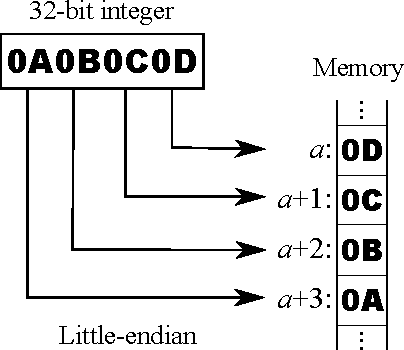
\includegraphics[width=0.8\textwidth]{little_endian}
            \end{center}
        \end{column}
    \end{columns}
    \sidenote{- Wikipedia}
\end{frame}

\section{Exploit printf}

\begin{frame}[fragile]{Death by \texttt{printf}}
    \begin{columns}
        \begin{column}{0.5\textwidth}
            \cfile[xleftmargin=0.8cm,firstline=4]{../format_string/main.c}
        \end{column}
        \begin{column}{0.5\textwidth}
            \pause
            \begin{pre*}{autogobble}
                ~> echo foobar | ./main
                You entered:
                foobar
            \end{pre*}
            \bigskip\pause
            \begin{pre*}{autogobble}
                ~> echo AAAABBBB | ./main
                correct
            \end{pre*}
            \bigskip\pause
            \begin{pre*} {autogobble}
                ~> echo '%08x' | ./main
                You entered:
                bfd98ed4
            \end{pre*}
            \medskip
            oh look, a pointer, this may come in handy
        \end{column}
    \end{columns}
\end{frame}

\begin{frame}{Death by \texttt{printf}}
    \begin{center}
        \huge Demonstration
    \end{center}
\end{frame}

\begin{frame}{Death by \texttt{printf}}
    \begin{itemize}
        \item Even functions which look very simple / basic can be exploited
        \medskip
        \item \texttt{printf} also allows you to \textbf{write} to memory
        \medskip
        \item RTFM
    \end{itemize}
\end{frame}

\section{Buffer Overflow}

\begin{frame}[fragile]{Variants}
    \begin{tabular}{p{0.5\textwidth} p{0.5\textwidth}}
        static memory corruption: &
        \begin{ccode*}{autogobble,linenos=false}
            static char buffer[64];
        \end{ccode*}
        \bigskip\\
        dynamic memory (heap) corruption: &
        \begin{ccode*}{autogobble,linenos=false}
            char *buffer = (char *) malloc(64);
            /* ... */
            free(buffer);
        \end{ccode*}
        \bigskip\\
        stack smashing: &
        \begin{ccode*}{autogobble,linenos=false}
            char buffer[64];
        \end{ccode*}
    \end{tabular}
\end{frame}

\begin{frame}{Smashing the Stack}
    \begin{columns}
        \begin{column}{0.5\textwidth}
            \begin{center}
                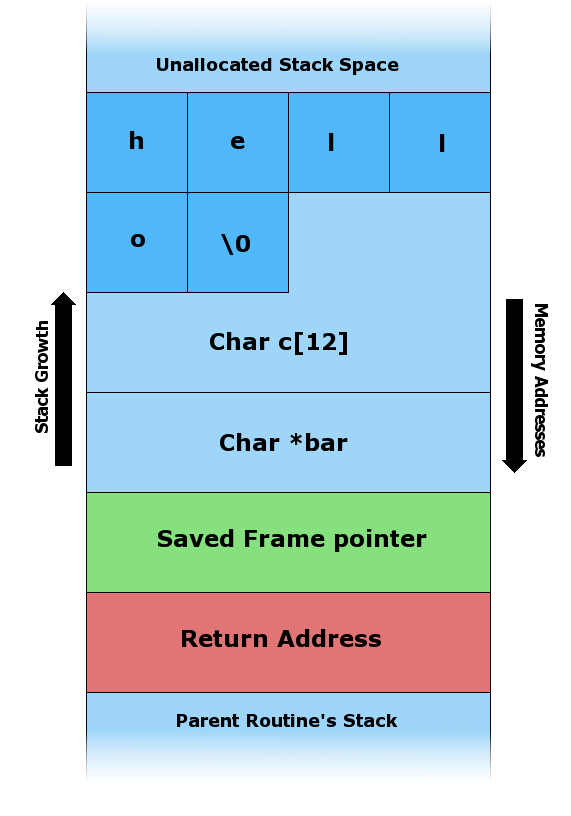
\includegraphics[width=0.75\textwidth]{stack_smash}
            \end{center}
        \end{column}
        \begin{column}{0.5\textwidth}
            \begin{itemize}
                \item Here, you write from top to bottom \bigskip
                \item You'll first overwrite local variables (\texttt{bar}) \bigskip
                \item Followed by arguments \bigskip
                \item Your \textbf{saved return address} \bigskip
                \item The next frame
            \end{itemize}
        \end{column}
    \end{columns}
    \sidenote{- Wikipedia}
\end{frame}

\begin{frame}{Overwrite a Flag}
    \begin{center}
        \huge Demonstration
    \end{center}
\end{frame}

\section{Shell Code}

\begin{frame}{Bend Return Address to jump into Buffer}
    \begin{center}
        \huge Demonstration
    \end{center}
\end{frame}

\section{Data Execution Prevention (DEP)}

\begin{frame}{Data Execution Prevention}
    \begin{columns}
        \begin{column}{0.5\textwidth}
            \begin{center}
                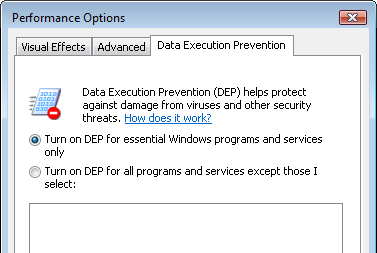
\includegraphics[width=0.9\textwidth]{dep_windows}
            \end{center}
        \end{column}
        \begin{column}{0.5\textwidth}
            \begin{itemize}
                \item also known as \textbf{write XOR execute} (\texttt{w\^{}x})
                \medskip
                \item sometimes called \textbf{page protection}
                \bigskip
                \item typically enforced by hardware
                \medskip
                \item \texttt{rwx} permissions per memory page
                \medskip
                \item \texttt{segfault} is triggered upon violation
            \end{itemize}
        \end{column}
    \end{columns}
\end{frame}

\begin{frame}{Data Execution Prevention}
    \begin{block}{Famous Quote}
        If your program simply segfaulted, consider yourself lucky.
    \end{block}
\end{frame}

\begin{frame}{Data Execution Prevention}
    \begin{itemize}
        \item We cannot bend the return address to the buffer anymore =(
        \item What now?
        \bigskip
        \pause
        \item Take control!
    \end{itemize}
\end{frame}

\begin{frame}{Return to a Different Function}
    \begin{center}
        \huge Demonstration
    \end{center}
\end{frame}

\section{Return Oriented Programming (ROP)}

\begin{frame}{Gadgets}

\end{frame}

\begin{frame}{Return to libC}

\end{frame}

\section{Address Space Layout Randomization (ASLR)}

\begin{frame}[fragile]{\texttt{/proc/self/maps}}
    \begin{pre*}{autogobble}
        ~> cat /proc/self/maps
        00400000-0040b000 r-xp 00000000 fc:01 1836175                            /bin/cat
        0060b000-0060c000 r--p 0000b000 fc:01 1836175                            /bin/cat
        0060c000-0060d000 rw-p 0000c000 fc:01 1836175                            /bin/cat
        00904000-00925000 rw-p 00000000 00:00 0                                  [heap]
        7fe33f33b000-7fe33f4fb000 r-xp 00000000 fc:01 5767649                    /lib/x86_64-linux-gnu/libc-2.21.so
        7ffc2bb0f000-7ffc2bb30000 rw-p 00000000 00:00 0                          [stack]
        7ffc2bb70000-7ffc2bb72000 r-xp 00000000 00:00 0                          [vdso]
    \end{pre*}
    \bigskip
    some lines have been omitted
\end{frame}
\begin{frame}[fragile]{\texttt{/proc/self/maps}}
    \begin{pre*}{autogobble}
        ~> cat /proc/self/maps
        00400000-0040b000 r-xp 00000000 fc:01 1836175                            /bin/cat
        0060b000-0060c000 r--p 0000b000 fc:01 1836175                            /bin/cat
        0060c000-0060d000 rw-p 0000c000 fc:01 1836175                            /bin/cat
        0240d000-0242e000 rw-p 00000000 00:00 0                                  [heap]
        7f3392f04000-7f33930c4000 r-xp 00000000 fc:01 5767649                    /lib/x86_64-linux-gnu/libc-2.21.so
        7ffdbee06000-7ffdbee27000 rw-p 00000000 00:00 0                          [stack]
        7ffdbeff5000-7ffdbeff7000 r-xp 00000000 00:00 0                          [vdso]
    \end{pre*}
    \bigskip
    some lines have been omitted
\end{frame}
\begin{frame}[fragile]{\texttt{/proc/self/maps}}
    \begin{pre*}{autogobble}
        ~> cat /proc/self/maps
        00400000-0040b000 r-xp 00000000 fc:01 1836175                            /bin/cat
        0060b000-0060c000 r--p 0000b000 fc:01 1836175                            /bin/cat
        0060c000-0060d000 rw-p 0000c000 fc:01 1836175                            /bin/cat
        00bd4000-00bf5000 rw-p 00000000 00:00 0                                  [heap]
        7f3f4ad4e000-7f3f4af0e000 r-xp 00000000 fc:01 5767649                    /lib/x86_64-linux-gnu/libc-2.21.so
        7fffc470e000-7fffc472f000 rw-p 00000000 00:00 0                          [stack]
        7fffc4766000-7fffc4768000 r-xp 00000000 00:00 0                          [vdso]
    \end{pre*}
    \bigskip
    some lines have been omitted
\end{frame}

\section{Heap Corruption}

\begin{frame}{Heap vs. Stack}
    \begin{itemize}
        \item Managed by the programmer through \texttt{malloc} /
            \texttt{calloc} / \texttt{recalloc} / \texttt{free}
        \medskip
        \item Mainly used for structs (objects), big buffers, persistent data
        \medskip
        \item \textbf{non-linear} structure
        \medskip
        \item Many different implementations (dlmalloc, ptmalloc, \dots)\\
            some applications come with their own implementation
        \medskip
        \item Details depend \emph{heavily} on implementation
    \end{itemize}
\end{frame}

\begin{frame}{Overflow}
    \begin{columns}
        \begin{column}{0.5\textwidth}
            \begin{center}
                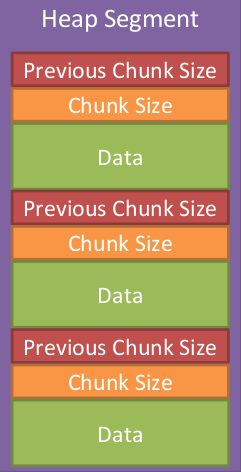
\includegraphics[height=0.9\textheight]{heap_segment}
            \end{center}
        \end{column}
        \begin{column}{0.5\textwidth}
            \begin{center}
                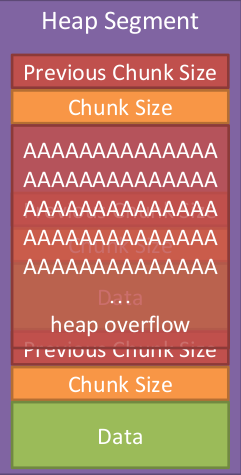
\includegraphics[height=0.9\textheight]{heap_overflow}
            \end{center}
        \end{column}
    \end{columns}
\end{frame}

\begin{frame}{Attack Surface}
    \begin{itemize}
        \item Anything that handles the now corrupted data can be viewed as
            additional attack surface
        \medskip
        \pause
        \item Structs commonly contain function pointers which can be
            overwritten
    \end{itemize}
\end{frame}

\section{Stack Cookies (Canary)}

\section{Code Pointer Integrity}

\section{A Word about x86\_64 and ARM}

\begin{frame}{Modern Devices}
    Your laptop, your server:
    \begin{itemize}
        \item likely x86\_64
    \end{itemize}
    \medskip
    \pause
    Your phone, your tablet, maybe even your watch:
    \begin{itemize}
        \item probably ARM
    \end{itemize}
    \medskip
    \pause
    Your router:
    \begin{itemize}
        \item probably MIPS
        \item maybe ARM somewhere in the future
    \end{itemize}
\end{frame}

\begin{frame}{About x86}
    \begin{itemize}
        \item no instruction alignment (great for ROP Gadgets)
        \item lot of instructions
        \item instruction length varies (\SIrange{1}{15}{\byte})
        \item \texttt{mov} is Turing Complete
    \end{itemize}
\end{frame}

\begin{frame}{About x64\_64}
    \begin{itemize}
        \item successor to x86
        \item also known as x64 or AMD64
        \item using fastcall calling convention
            \begin{itemize}
                \item some arguments put into registers (\texttt{RDI},
                    \texttt{RSI}, \texttt{RDX}, \texttt{RCX}, \texttt{R8},
                    \texttt{R9})
                \item this makes ROP much easier
            \end{itemize}
        \item more entropy for ASLR (hard to bruteforce)
    \end{itemize}
\end{frame}

\begin{frame}{About ARM}
    \begin{itemize}
        \item used in \emph{low power} devices
        \item smaller number of registers (though \SI{32}{\bit})
        \item calling convention similar to fastcall (\texttt{r0}, \texttt{r1},
            \texttt{r2}, \texttt{r3})
        \item instructions can work on multiple registers at once
        \item special \SI{16}{\bit} mode (\textbf{THUMB})
        \item cache not flushed automatically
    \end{itemize}
\end{frame}

\section{Fuzzing}

\section{Polymorphic Code}

\begin{frame}{Polymorphism}
    \begin{center}
        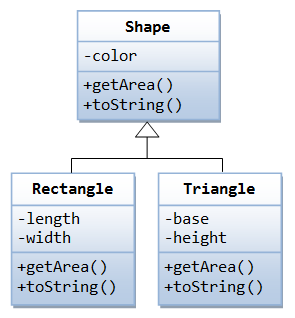
\includegraphics[height=0.7\textheight]{polymorphism}
    \end{center}
    \sidenote{\url{- ntu.edu.sg}}
\end{frame}

\begin{frame}{\st{Polymorphism} Polymorphic Code}
    \begin{itemize}
        \item code which \emph{evolves} during runtime
        \item often malicious code, but also used in DRM
        \item makes use of encryption
        \medskip
        \pause
        \item makes static analysis hard, you basically need to reverse
            engineer the system,\\
            running it may not reveal all parts or be straight up lethal!
    \end{itemize}
\end{frame}

\begin{frame}{\st{Polymorphism} Polymorphic Code}
    \begin{itemize}
        \item malicious parts sometimes only triggered when special conditions
            are met (time, platform, events, \dots)
        \medskip
        \pause
        \item \textbf{metamorphic engines} are used to generated new code;\\
            little documentation / public knowledge;\\
            some even see it as taboo
        \medskip
        \pause
        \item have a look at \url{http://z0mbie.daemonlab.org/}\\
            and \url{http://vxheaven.org/lib/vmd01.html}
    \end{itemize}
\end{frame}

\begin{frame}[t,fragile]{Hijack Example (last year)}
    \begin{columns}
        \begin{column}{0.75\textwidth}
            \cfile[xleftmargin=0.8cm,firstline=8,lastline=26]{../hijack/main.c}
        \end{column}
        \begin{column}{0.25\textwidth}
            \cfile[xleftmargin=0.8cm,firstline=28,lastline=42]{../hijack/main.c}
        \end{column}
    \end{columns}
\end{frame}

\section*{Conclusion}

\begin{frame}{Fin.}
   \begin{center}
       \huge OMG finally\dots
   \end{center}
\end{frame}

\begin{frame}{``But I use Java!''}
    \begin{center}
        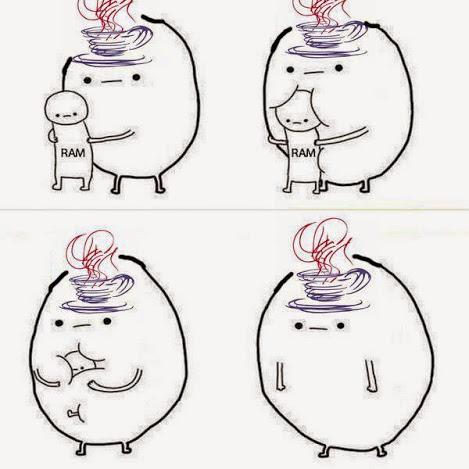
\includegraphics[height=0.9\textheight]{jvm_ram}
    \end{center}
    \sidenote{- \url{http://twitter.com/java_monitor}}
\end{frame}

\begin{frame}{``But I use Java!''}
    Don't worry, we got you covered.

    \bigskip

    There are a lot of different exploits out there, which share a lot of
    similarities.

    \bigskip

    Have a look at this: \url{http://foxglovesecurity.com/2015/11/06/}
\end{frame}

\end{document}
